\chapter{生物体：与其环境相互作用的系统}\label{ch:b1:organism-environment}

一月的一个清晨，一只兔子坐在草地边缘。接下来的
一小时里，它将吃掉一百克草，呼吸约 \qty{400}{L} 的
空气，经皮毛向 \qty{2}{\celsius} 的空气散热，在水洼边
饮水，并在鹰的影子掠过原野时猛然窜逃。它的任何活动
都离不开某物穿过其边界：物质进入与
排出，能量进出，信息进入。两百米外，一棵橡树
不必移动，却做着同样的事——吸收二氧化碳和光，
通过比树冠还大的根系吸取水分，并将这些水分
散失到同样寒冷的空气中。本章阐明\omterm{def:b1:organism-environment:organism}{生物体}作为一个系统是什么，
为何其大小决定了它的构造，外界不断变化时它如何保持内部稳定，
以及其能量需求如何随
质量而变化。本开篇的两种生物，一种哺乳动物和一种
开花植物，是全学年反复回到的模型。

\begin{omfigure}
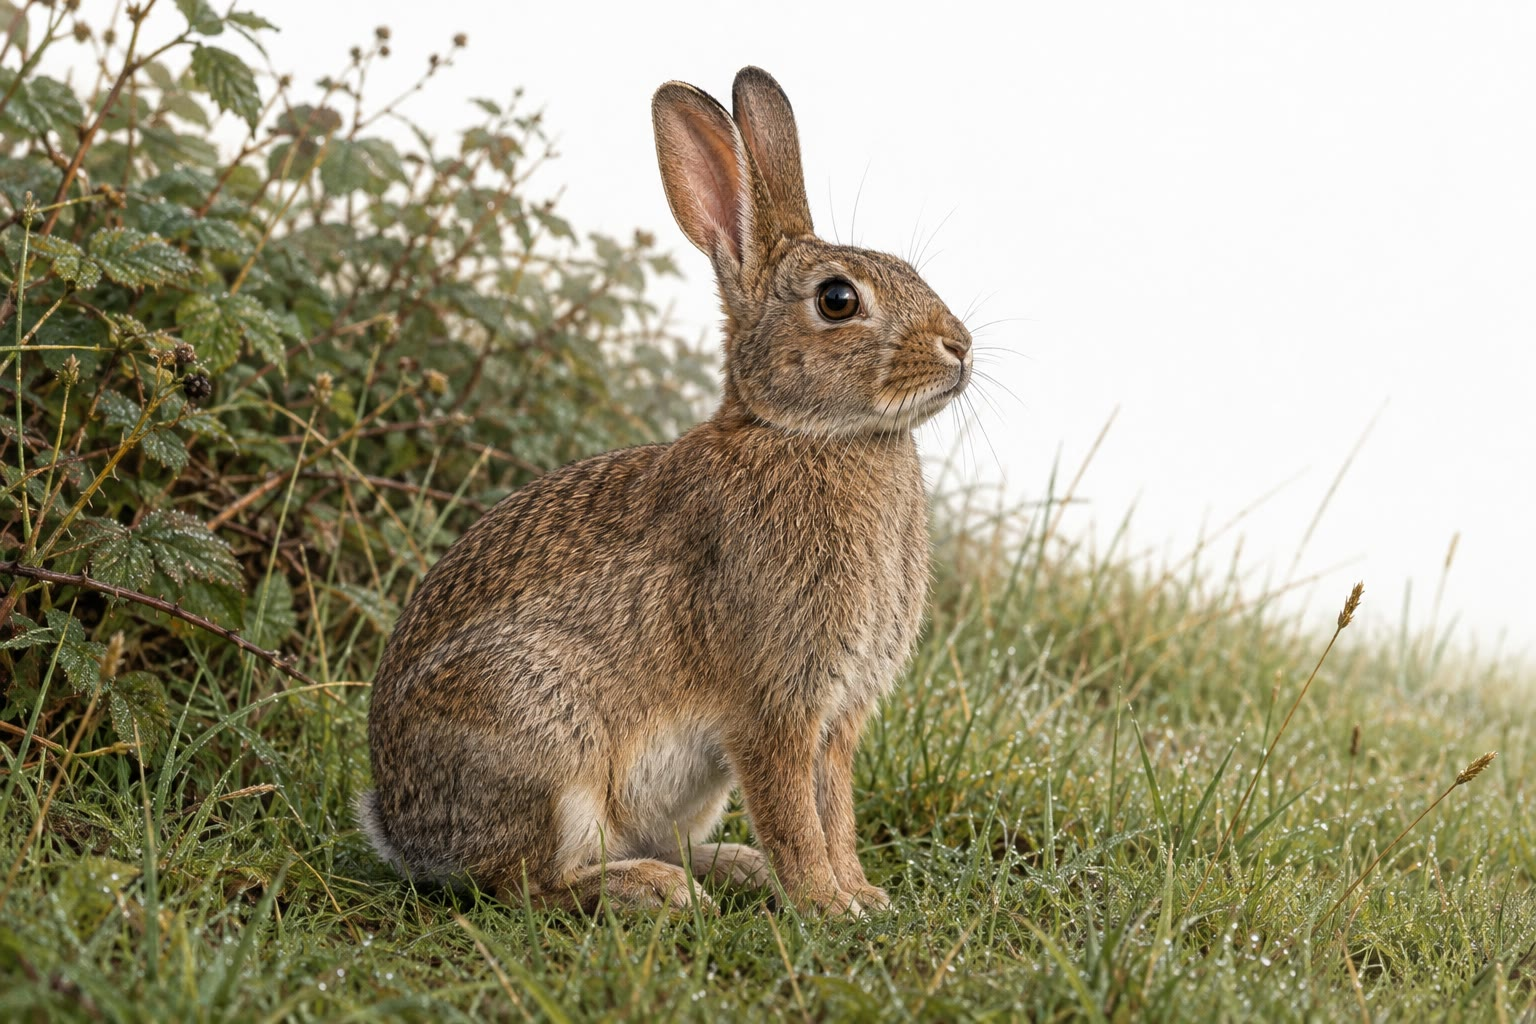
\includegraphics[width=0.62\linewidth]{images/book3/ai/b3-01-rabbit-field.jpg}

{\small 草地边缘的一只野兔：一小时内它将进食、
呼吸、散热、饮水和逃逸——每一项都是
穿越其边界的一次交换。}
\end{omfigure}

\section{开口系统}

\begin{definition}[生物体，开口系统]\label{def:b1:organism-environment:organism}
称\emph{生物体}\index{生物体}为一个活的个体：具有边界、
能够自我维持和自我繁殖的系统，由一个细胞或多个细胞组成，
这些细胞具有共同的起源和共同的功能。它是一个
\emph{开口系统}\index{开口系统}：物质和能量穿过其
边界并持续进行，它只有在交换持续时才能维持生命。生物体的
\emph{环境}\index{环境}是指边界之外
与其发生交换的一切事物，包括物理介质
（空气、水、土壤、光、温度）以及其他生物体。
\end{definition}

\begin{proposition}[三种交换]\label{prop:b1:organism-environment:exchanges}
每个\omterm{def:b1:organism-environment:organism}{生物体}都与其\omterm{def:b1:organism-environment:organism}{环境}交换三类事物：
\begin{itemize}
  \item \emph{物质}\index{物质交换}：吸收营养物质、
        水和气体，并释放废物、气体和水；
  \item \emph{能量}\index{能量交换}：以光（\omterm{def:b1:organism-environment:trophy}{自养}生物）
        或食物的化学能（\omterm{def:b1:organism-environment:trophy}{异养}生物）形式吸收能量，
        并几乎全部以热量形式释放；
  \item \emph{信息}\index{信息交换}：检测\omterm{def:b1:organism-environment:organism}{环境}中的信号
        （光、化学物质、温度、
        触觉、声音），并对其作出响应。
\end{itemize}
在\omterm{def:b1:organism-environment:organism}{生物体}既不生长也不缩小的时段内，其
收支是平衡的：输入的物质等于输出的物质，输入的能量
等于输出的热量加上对外做的功。
\end{proposition}
\begin{proof}
前两条由应用于边界内部体积的质量守恒与能量守恒得出：
凡是积累起来的，都是输入与输出之差，
而稳定的\omterm{def:b1:organism-environment:organism}{生物体}不积累任何东西。
未被储存为新生物量的化学能最终变为热量，因为
\omterm{def:b1:organism-environment:organism}{生物体}的每一个反应都以热量形式耗散其自由能，并且
对外做的机械功（运动、举起）是唯一的
另一条去向。第三条依据的观察是：没有任何\omterm{def:b1:organism-environment:organism}{生物体}对
其周围\omterm{def:b1:organism-environment:organism}{环境}无动于衷。
\end{proof}

\begin{omfigure}
\begin{tikzpicture}[font=\footnotesize, >=Stealth, line cap=round]
  \draw[very thick, omDef, fill=omDef!6, rounded corners=12pt] (0,0) rectangle (4.4,3.4);
  \node[font=\small\bfseries, omDef] at (2.2,2.95) {生物体};
  \node[align=center] at (2.2,1.5) {内环境 \\ 细胞、组织、器官 \\ 化学做功、生长、\\ 运动、繁殖};
  % matter in / out
  \draw[->, thick, omProp] (-1.3,2.6) -- (0,2.6) node[pos=0, left, align=right] {营养物质、水、\\ $\mathrm{O_2}$ 或 $\mathrm{CO_2}$};
  \draw[->, thick, omProp] (4.4,2.6) -- (5.7,2.6) node[right, align=left] {废物、水、\\ $\mathrm{CO_2}$ 或 $\mathrm{O_2}$};
  % energy
  \draw[->, thick, omThm] (-1.3,1.5) -- (0,1.5) node[pos=0, left, align=right] {能量：光，或 \\ 食物的化学能};
  \draw[->, thick, omThm] (4.4,1.5) -- (5.7,1.5) node[right, align=left] {热量，以及 \\ 对外做的功};
  % information
  \draw[->, thick, omExo] (-1.3,0.5) -- (0,0.5) node[pos=0, left, align=right] {信息：光、\\ 化学物质、温度};
  \draw[->, thick, omExo] (4.4,0.5) -- (5.7,0.5) node[right, align=left] {响应：运动、\\ 分泌、生长};
\end{tikzpicture}

{\small 作为\omterm{def:b1:organism-environment:organism}{开口系统}的\omterm{def:b1:organism-environment:organism}{生物体}：物质（橙色）、能量（红色）和
信息（绿色）穿过其边界。稳定的\omterm{def:b1:organism-environment:organism}{生物体}释放的
物质与其吸收的一样多，并将几乎全部能量摄入转化为
热量。}
\end{omfigure}

\begin{definition}[自养，异养]\label{def:b1:organism-environment:trophy}
若\omterm{def:b1:organism-environment:organism}{生物体}借助外界能源，由无机碳（二氧化碳）构建
自身的有机物，则称其为\emph{自养}\index{自养}。以光为能源的是
\emph{光能自养生物}\index{光能自养生物}（植物、藻类、蓝细菌），
以无机化合物氧化为能源的，
则是\emph{化能自养生物}\index{化能自养生物}。
若生物必须摄取其他生物制造的有机物，则称其为\emph{异养}\index{异养}。
这些有机物既提供碳，也提供能量
（动物、真菌以及大多数细菌）。
\end{definition}

\begin{example}[兔子与橡树]\label{ex:b1:organism-environment:rabbitoak}
兔子消化后的一百克草，约可提供
\qty{500}{kJ} 的化学能，以及它将要构建的每个分子中的碳；
其呼吸所吸入的氧气使它能够氧化这些食物，而它
呼出的二氧化碳正是同一种碳离开体外。橡树的摄入则
恰好相反：吸入二氧化碳，释放氧气，能量以光的形式进入
——正午时约 \qty{5}{kW} 的光照射在其树冠上，其中它储存的
不到百分之一以糖的形式储存。两者几乎都以热量形式释放
其所处理的全部能量：兔子的皮毛是温热的，橡树的叶片则
由其自身吸光所驱动的蒸发而降温。
\end{example}

\section{组织层次与大小问题}

\begin{definition}[组织层次]\label{def:b1:organism-environment:levels}
生命物质按嵌套的
\emph{组织层次}\index{组织层次}排列，每一层都由其下一层的单元构成，
并具有下层所没有的性质：
分子（$\qty{1}{nm}$）、细胞（$\qtyrange{1}{100}{\micro m}$）、
组织、器官（$\qtyrange{1}{100}{mm}$）、器官系统、\omterm{def:b1:organism-environment:organism}{生物体}
（$\qty{1}{\micro m}$ 至 $\qty{100}{m}$），再往上依次是种群、
群落、生态系统和生物圈。细胞进行呼吸作用，而
分子则不能。种群会演化，\omterm{def:b1:organism-environment:organism}{生物体}则不会。
\end{definition}

\begin{proposition}[表面与体积]\label{prop:b1:organism-environment:sv}
对形状相同、特征尺寸为 $L$ 的物体，表面积
按 $L^2$ 增长，体积按 $L^3$ 增长，因此表面积与体积之比
按 $1/L$ 减小：
\[
\frac{S}{V} \propto \frac{1}{L}, \qquad
\frac{S}{V}\Big|_{\text{球}} = \frac{4\pi r^2}{\tfrac{4}{3}\pi r^3} = \frac{3}{r}.
\]
\omterm{def:b1:organism-environment:organism}{生物体}所交换的一切都要穿过一个表面，而它
所消耗的一切都与其体积成正比：大型\omterm{def:b1:organism-environment:organism}{生物体}无法
仅凭外表面供给其整个体积。
\end{proposition}
\begin{proof}
将形状按比例因子 $k$ 放大，每个面积变为原来的 $k^2$ 倍，每个
体积变为 $k^3$ 倍；比值变为原来的 $1/k$ 倍。对于球体，
该公式是精确的。
\end{proof}

\begin{example}[细菌与人]\label{ex:b1:organism-environment:svnumbers}
半径为 $\qty{0.5}{\micro m}$ 的细菌，其
$S/V = 3/r = \qty{6e6}{m^{-1}}$：其细胞质中每立方微米都
距离外界不超过半微米，通过其
膜的扩散即可完全满足其需要。若将人体看作体积为 \qty{70}{L} 的球体，
则 $r = \qty{0.26}{m}$，$S/V = \qty{12}{m^{-1}}$，仅为前者的
五十万分之一。皮肤面积约 \qty{2}{m^2}，无法供应
\qty{70}{kg} 组织所消耗的氧气；肺折叠于胸腔之内，
表面积达 \qty{100}{m^2}，肠道则经三重折叠，
表面积为 \qty{30}{m^2}。
\end{example}

\begin{omfigure}
\begin{tikzpicture}
\begin{axis}[
  xbar, bar width=8pt,
  width=0.82\linewidth, height=6.2cm,
  axis x line=bottom, axis y line=left,
  xmode=log, log origin=infty, xmin=0.5, xmax=3000,
  xlabel={交换表面积（\unit{m^2}）},
  xlabel style={font=\small, at={(axis description cs:0.5,-0.13)}, anchor=north},
  symbolic y coords={human skin, human lung, human small intestine, oak leaves, rye root system, rye root hairs},
  ytick=data, yticklabels={人的皮肤, 人的肺, 人的小肠, 橡树叶, 黑麦根系, 黑麦根毛}, tick label style={font=\small},
  enlarge y limits=0.12,
  nodes near coords, nodes near coords style={font=\scriptsize, anchor=west},
  point meta=rawx,
]
\addplot[fill=omDef!45, draw=omDef] coordinates
  {(2,human skin) (100,human lung) (30,human small intestine) (300,oak leaves) (240,rye root system) (400,rye root hairs)};
\end{axis}
\end{tikzpicture}

{\small 交换表面，对数刻度。人体的外表面积为
\qty{2}{m^2}；人体内部折叠的表面，以及
植物伸入空气和土壤中的表面，则大了十到两百倍。
（一株黑麦在箱中培育四个月：根的面积为 \qty{240}{m^2}，
根毛的面积为 \qty{400}{m^2}。）}
\end{omfigure}

\begin{proposition}[交换表面具有折叠、薄和通风的特点]\label{prop:b1:organism-environment:surfaces}
体长超过约一毫米时，\omterm{def:b1:organism-environment:organism}{生物体}无法仅靠
经外表面的扩散获得养分。任何大小的多细胞\omterm{def:b1:organism-environment:organism}{生物体}
因此都具有\emph{特化的交换表面}\index{交换表面}，其共同的设计以四种方式解决同一问题：一是大面积
（折叠：绒毛、肺泡、鳃小片、根毛、叶
片），二是薄的厚度（两介质之间仅一层细胞甚至更薄），
三是外侧介质不断更新（通风、水流、
蒸腾流），四是内部具有运输系统（血液、
汁液），将穿过表面的物质运送至整个体积的其余部分。
\end{proposition}
\begin{proof}
菲克定律（见\cref{ch:b1:membranes-transport}）给出穿过一个
表面的通量与面积、浓度差成正比，并与
厚度的倒数成正比；更新外侧介质使
浓度差保持较大；运输系统移走已穿过的物质，
并使内侧浓度保持较低。四个特征中的每一个都
增大通量，大型\omterm{def:b1:organism-environment:organism}{生物体}需要全部四项。
\end{proof}

\section{内环境与稳态}

\begin{definition}[内环境]\label{def:b1:organism-environment:milieu}
在多细胞动物中，大多数细胞并不直接与外界接触，
而是浸浴于\emph{内环境}\index{内环境}之中：细胞外液（血浆、淋巴液、
细胞间的组织液），其成分、温度和
体积受\omterm{def:b1:organism-environment:organism}{生物体}调节。细胞与该液体交换物质；该液体
再经\omterm{prop:b1:organism-environment:surfaces}{特化的交换表面}与外界交换物质。
这一思想出自克洛德·贝尔纳（1865）：内\omterm{def:b1:organism-environment:organism}{环境}
的恒定是自由而独立生活的条件。
\end{definition}

\begin{definition}[稳态]\label{def:b1:organism-environment:homeostasis}
\emph{稳态}\index{稳态}是指将\omterm{def:b1:organism-environment:milieu}{内环境}中受调节的
变量（温度、葡萄糖
浓度、pH、渗透压、血压）维持在接近
\emph{调定点}\index{调定点}附近，不受外界变化影响。它通过
\emph{负反馈}\index{负反馈}实现：一个
\emph{感受器}测量该变量，整合中枢将其与
调定点比较，\emph{效应器}朝着
抵消偏差的方向发挥作用。该变量并非固定不变，而是在
调定点周围的一个狭窄范围内波动。
\end{definition}

\begin{omfigure}
\begin{tikzpicture}[font=\small, >=Stealth, line cap=round,
  box/.style={draw, thick, rounded corners=4pt, minimum height=9mm, minimum width=26mm, align=center, fill=white}]
  \node[box, fill=omDef!10] (var) at (0,0) {受调节的变量 \\ （例如体温）};
  \node[box, fill=omProp!10] (sens) at (4.6,1.5) {感受器 \\ （温度感受器）};
  \node[box, fill=omThm!10] (int) at (4.6,-1.5) {整合中枢 \\ （下丘脑）};
  \node[box, fill=omExo!10] (eff) at (0,-3.0) {效应器 \\ （寒战、血管、汗液）};
  \node[font=\footnotesize, align=center] (set) at (8.4,-1.5) {调定点 \\ $\qty{37}{\celsius}$};
  \draw[->, thick] (var.east) -- ++(1.0,0) |- (sens.west);
  \draw[->, thick] (sens.south) -- (int.north) node[midway, right, font=\footnotesize] {测量值};
  \draw[->, thick] (set.west) -- (int.east);
  \draw[->, thick] (int.south) -- ++(0,-0.6) -| (eff.east) ;
  \draw[->, thick] (eff.north) -- (var.south) node[midway, left, font=\footnotesize, align=right] {纠正，\\ 与偏差方向相反};
  \draw[->, thick, gray] (-3.6,0.9) -- (var.north west) node[pos=0, above, font=\footnotesize, gray, align=center] {干扰 \\ （冷空气）};
\end{tikzpicture}

{\small \omterm{def:b1:organism-environment:homeostasis}{负反馈}回路。感受器报告该变量的数值，
中枢将其与\omterm{def:b1:organism-environment:homeostasis}{调定点}比较，效应器则推动变量回到原处。
纠正作用总与偏差
的方向相反——因此称为\emph{负}反馈。}
\end{omfigure}

\begin{proposition}[内温动物与外温动物]\label{prop:b1:organism-environment:thermo}
\emph{外温动物}\index{外温动物}（大多数无脊椎动物、鱼类、
两栖动物、爬行动物）的体温随\omterm{def:b1:organism-environment:organism}{环境}变化，
其\omterm{def:b1:organism-environment:allometry}{代谢率}随温度升高而上升，
大约每升高 \qty{10}{\celsius} 翻一番。\emph{内温动物}\index{内温动物}
（哺乳动物、鸟类）通过代谢产热，将体温维持在\omterm{def:b1:organism-environment:homeostasis}{调定点}。
在\omterm{def:b1:organism-environment:organism}{环境}温度处于
\emph{热中性区}\index{热中性区}范围内时，它以基础速率代谢，
仅通过调节隔热层和皮肤血流来调整；
低于该区间时，其\omterm{def:b1:organism-environment:allometry}{代谢率}随气温下降而线性上升，
因为散热与温差成正比，
必须由产热来抵消；高于该区间时，蒸发散热要消耗
水分和能量。
\end{proposition}
\begin{proof}[部分证明]
对于温度为 $T_b$ 的物体，置于温度为 $T_a$ 的空气中，
单位时间内经其表面散失的热量为 $P = hS\,(T_b - T_a)$（牛顿冷却定律），其中 $h$
为因皮毛、羽毛或脂肪而降低的系数。
稳定的体温要求产热量等于 $P$，因此在\omterm{prop:b1:organism-environment:thermo}{热中性区}以下，产热量关于 $T_a$ 为线性，
斜率为 $-hS$。\omterm{prop:b1:organism-environment:thermo}{热中性区}的存在及其宽度
（其中 $h$ 本身被调节，如竖起皮毛、收缩皮肤血管）
是生理事实，而不是该方程的推论。
\end{proof}

\begin{omfigure}
\begin{tikzpicture}
\begin{axis}[
  width=0.9\linewidth, height=6.4cm,
  axis x line=bottom, axis y line=left,
  xmin=-10, xmax=45, ymin=0, ymax=5.2,
  xlabel={环境温度（\unit{\celsius}）}, ylabel={代谢率（基础代谢的倍数）},
  xlabel style={font=\small, at={(axis description cs:0.5,-0.12)}, anchor=north},
  ylabel style={font=\small},
  tick label style={font=\small}, xtick={-10,0,10,20,30,40}, ytick={1,2,3,4,5},
  clip=false, legend style={font=\small, at={(0.97,0.97)}, anchor=north east, draw=none},
]
\addplot[very thick, omThm] coordinates {(-10,4.6) (0,3.4) (10,2.2) (20,1.0) (30,1.0) (33,1.05) (38,1.5) (42,2.2)};
\addlegendentry{内温动物（小鼠）}
\addplot[very thick, omDef] coordinates {(-10,0.05) (0,0.12) (10,0.25) (20,0.5) (30,1.0) (40,2.0)};
\addlegendentry{外温动物（蜥蜴）}
\draw[dashed, gray] (axis cs:20,0) -- (axis cs:20,1.0);
\draw[dashed, gray] (axis cs:30,0) -- (axis cs:30,1.0);
\node[font=\scriptsize, anchor=south, align=center] at (axis cs:25,1.15) {热中性 \\ 区};
\node[font=\scriptsize, anchor=west, align=left] at (axis cs:11,3.5) {斜率 $= -hS$：产热 \\ 与散热相等};
\end{axis}
\end{tikzpicture}

{\small \omterm{def:b1:organism-environment:allometry}{代谢率}与\omterm{def:b1:organism-environment:organism}{环境}温度的关系。\omterm{prop:b1:organism-environment:thermo}{内温动物}的\omterm{def:b1:organism-environment:allometry}{代谢率}
在\omterm{prop:b1:organism-environment:thermo}{热中性区}内最低，气温下降时线性上升；
\omterm{prop:b1:organism-environment:thermo}{外温动物}的\omterm{def:b1:organism-environment:allometry}{代谢率}则简单地随温度变化，
每升高十度翻一番。}
\end{omfigure}

\begin{example}[两度的一夜]\label{ex:b1:organism-environment:night}
开篇提到的那只兔子在洞穴中静息，在\omterm{prop:b1:organism-environment:thermo}{热中性区}内产热约
\qty{6}{W}。外界气温为
\qty{2}{\celsius}，比该区间下限低二十度，
其产热必须升至约 \qty{12}{W}：寒战与
脂肪储备的氧化提供了这部分差额，而其觅食
时间随之延长。同一河岸上的蜥蜴不与寒冷抗争：其
体温降至 \qty{3}{\celsius}，代谢降至夏季水平的
二十分之一，直到太阳重新升起才会活动。
\end{example}

\section{代谢率与体重}

\begin{definition}[代谢率，异速生长]\label{def:b1:organism-environment:allometry}
\omterm{def:b1:organism-environment:organism}{生物体}的\emph{代谢率}\index{代谢率} $B$ 是指其转化化学能的速率，
以瓦特计，可用产热量表示，
也可用耗氧量表示（$\qty{1}{L}$ 的 $\mathrm{O_2}$
消耗 $\approx \qty{20}{kJ}$）。\emph{基础代谢率}\index{基础代谢率}
是静息、禁食的\omterm{prop:b1:organism-environment:thermo}{内温动物}
在\omterm{prop:b1:organism-environment:thermo}{热中性区}时的代谢率。若量 $Y$ 随体重\emph{异速地}\index{异速生长}变化，
记体重为 $M$，
即 $Y = a\,M^{b}$，指数 $b \neq 1$；在对数—对数图上，该关系为
斜率为 $b$ 的直线。
\end{definition}

\begin{theorem}[克莱伯定律]\label{thm:b1:organism-environment:kleiber}
\index{克莱伯定律}
从尖鼠到鲸，哺乳动物与鸟类的\omterm{def:b1:organism-environment:allometry}{基础代谢率}
与体重的四分之三次幂成正比：
\[
B \approx \qty{3.4}{W}\times\left(\frac{M}{\qty{1}{kg}}\right)^{3/4}.
\]
因此，\emph{质量比\omterm{def:b1:organism-environment:allometry}{代谢率}} $B/M$ 随 $M^{-1/4}$ 下降：每克
小家鼠燃烧能量的速度，约为每克
大象的二十倍。
\end{theorem}
\begin{proof}[证据]
克莱伯（1932 年）将体重 \qty{20}{g} 至 \qty{600}{kg} 之间动物的实测产热量
对其体重作双对数图，
得到一条斜率为 $0.74$ 的直线，而不是
表面积比例散热所预言的 $0.67$。此后，该直线已
延伸至跨越八个数量级的质量范围，斜率
在几个百分点之内保持不变。指数为何是 $3/4$ 而非 $2/3$
仍有争议：目前主流的解释将其与
向每个细胞输送氧气的分支网络（血管、气道）的几何结构相联系。
\end{proof}

\begin{omfigure}
\begin{tikzpicture}
\begin{loglogaxis}[
  width=0.9\linewidth, height=6.6cm,
  axis x line=bottom, axis y line=left,
  xmin=0.005, xmax=20000, ymin=0.05, ymax=6000,
  xlabel={体重 (\unit{kg})}, ylabel={基础代谢率 (\unit{W})},
  xlabel style={font=\small, at={(axis description cs:0.5,-0.12)}, anchor=north},
  ylabel style={font=\small},
  tick label style={font=\small},
  xtick={0.01,0.1,1,10,100,1000,10000}, ytick={0.1,1,10,100,1000},
  log ticks with fixed point,
  clip=false,
]
\addplot[thick, omThm, domain=0.005:20000, samples=40] {3.4*x^0.75};
\addplot[only marks, mark=*, mark size=2pt, omDef] coordinates
  {(0.02,0.19) (0.3,1.3) (3,7.5) (70,80) (500,360) (4000,1700)};
\node[font=\scriptsize, anchor=west] at (axis cs:0.02,0.19) {\ 小鼠};
\node[font=\scriptsize, anchor=west] at (axis cs:0.3,1.3) {\ 大鼠};
\node[font=\scriptsize, anchor=west] at (axis cs:3,7.5) {\ 猫};
\node[font=\scriptsize, anchor=west] at (axis cs:70,80) {\ 人};
\node[font=\scriptsize, anchor=west] at (axis cs:500,360) {\ 马};
\node[font=\scriptsize, anchor=north] at (axis cs:4000,1300) {大象};
\node[font=\scriptsize, anchor=south east, omThm] at (axis cs:8000,4000) {斜率 $3/4$};
\end{loglogaxis}
\end{tikzpicture}

{\small \omterm{thm:b1:organism-environment:kleiber}{克莱伯定律}。六种哺乳动物的\omterm{def:b1:organism-environment:allometry}{基础代谢率}与体重的关系，
在双对数坐标下作图：各点落在斜率为 $3/4$ 的直线上，
在跨越五个数量级的质量范围内成立。}
\end{omfigure}

\begin{method}[读取异速图]\label{met:b1:organism-environment:loglog}
\begin{enumerate}
  \item 以 $\log Y$ 对 $\log M$ 作图（或使用对数坐标轴）。
        幂律 $Y = aM^b$ 化为直线 $\log Y = \log a + b\log M$。
  \item 指数 $b$ 即斜率：在 $M$ 上取相差一个数量级的两点，
        $b$ 为 $Y$ 所升高的数量级个数。
        指数为 $1$ 表示正比关系（等速性）；$b < 1$ 时，
        该量增长慢于质量；$b > 1$ 时，增长快于质量。
  \item 系数 $a$ 是 $Y$ 在 $M = 1$ 处的值（此时
        $\log M = 0$）。
  \item 比较两种生物时，用比值：$Y_2/Y_1 =
        (M_2/M_1)^b$。按单位质量计，指数变为 $b-1$。
\end{enumerate}
\end{method}

\begin{example}[小鼠与大象]\label{ex:b1:organism-environment:mouseelephant}
一只 \qty{20}{g} 的小鼠：$B = 3.4\times 0.02^{0.75} = \qty{0.18}{W}$，或
\qty{9}{W/kg}。一头 \qty{4}{t} 的大象：$B = 3.4\times 4000^{0.75} =
\qty{1700}{W}$，或 \qty{0.43}{W/kg}。大象的耗能约为小鼠的一万倍，
但其每克组织的耗能却少了二十一倍，
即 $(4000/0.02)^{-1/4} = 1/21$。小鼠每天须进食相当于其体重十分之一的食物，
大象则只需五十分之一。小鼠的心脏每分钟跳动
\qty{600}{} 次，大象则为 \qty{30}{} 次：心率与
$B/M$ 一样，按 $M^{-1/4}$ 标度变化，而两者的心脏
在一生中都大约跳动十亿次。
\end{example}

\begin{remark}[两种标度指数及其推论]\label{rem:b1:organism-environment:consequences}
\omterm{def:b1:organism-environment:organism}{生物体}的许多速率按 $M^{-1/4}$ 标度变化（心率、呼吸
频率、单位质量\omterm{def:b1:organism-environment:allometry}{代谢率}），许多时间则按 $M^{+1/4}$ 标度变化（寿命、
妊娠期、达到成熟的时间）；它们的乘积，例如一生中的心跳次数，
因此与质量无关。器官的大小接近按
$M^{1}$ 标度变化（心脏、肺和血量都占体重的固定比例），
而进行交换的表面则按 $M^{3/4}$ 标度变化——
这就是为什么大型动物的肺比小型动物的肺更精细地折叠，
而不仅仅是更大。
\end{remark}

\section{两种模式生物}

\begin{proposition}[一种哺乳动物与一种开花植物]\label{prop:b1:organism-environment:models}
本学年用作模型的两类多细胞生物，以相反的方式解决上述
问题。哺乳动物是一种能动的\omterm{def:b1:organism-environment:trophy}{异养}生物，具有受调节的
\omterm{def:b1:organism-environment:milieu}{内环境}：它通过寻找并进食获取物质与能量，
经由循环系统供应的内表面（肠道、肺、肾）进行交换，
并使体温与血液成分保持恒定，最终达到固定的
成体形态。开花植物则是一种固着的\omterm{def:b1:organism-environment:trophy}{光能自养生物}，具有开放的
模块化身体：它在叶片处从光和空气中获取能量与碳，
在根部从土壤中获取水分与无机盐，经由
外表面进行交换，并在一生中不断通过生长扩大这些表面；
它不调节自身温度，
其形态随所处的位置而调整。
接下来的两章将分别描述二者。
\end{proposition}

\begin{example}[同一小时，两种收支]\label{ex:b1:organism-environment:budgets}
在开篇的那一小时里，兔子把 \qty{500}{kJ} 的草
转化为热量、运动以及少量生长，同时将血液温度维持在 \qty{39}{\celsius}，
将葡萄糖浓度维持在 \qty{6}{mmol/L} 附近；它是通过移动到食物处做到这一点的。
橡树把树冠所接收的几百千焦阳光转化为糖，
为此经叶片散失了 \qty{5}{L} 水，
并长出了几微米厚的新木质部；它是通过处在光与水充足的地方做到这一点的。
两者都是开放系统；两者都借助交换维持自身运转；
它们交换的方式，
正是它们生活的方式。
\end{example}

\section{练习}

\begin{exercise}[$\star$]\label{exo:b1:organism-environment:1}
说出\omterm{def:b1:organism-environment:organism}{生物体}与其
\omterm{def:b1:organism-environment:organism}{环境}之间的三种交换类型，并分别给出哺乳动物和植物各一个例子。
\end{exercise}

\begin{exercise}[$\star$]\label{exo:b1:organism-environment:2}
说明当一个球形细胞的半径加倍时，
其表面积与体积之比如何变化，并说明为何这限制了细胞的大小。
\end{exercise}

\begin{exercise}[$\star$]\label{exo:b1:organism-environment:3}
定义\omterm{def:b1:organism-environment:homeostasis}{稳态}，并说出\omterm{def:b1:organism-environment:homeostasis}{负反馈}回路的三个组成部分，
并指出它们在体温调节中分别对应什么。
\end{exercise}

\begin{exercise}[$\star$]\label{exo:b1:organism-environment:4}
根据\omterm{def:b1:organism-environment:allometry}{代谢率}图，蜥蜴的\omterm{def:b1:organism-environment:allometry}{代谢率}在
\qty{30}{\celsius} 与 \qty{10}{\celsius} 之间下降了多少倍，
而小鼠的\omterm{def:b1:organism-environment:allometry}{代谢率}在 \qty{20}{\celsius} 与
\qty{0}{\celsius} 之间上升了多少倍？
\end{exercise}

\begin{exercise}[$\star\star$]\label{exo:b1:organism-environment:5}
一个边长为 \qty{1}{mm} 的立方体形\omterm{def:b1:organism-environment:organism}{生物体}，每秒每立方毫米需要
\qty{1}{nmol} 氧气，其表面每平方毫米至多能以
\qty{2}{nmol/s} 的速率吸收氧气。它能否仅靠通过表面的扩散而生存？
对边长为 \qty{10}{mm} 的\omterm{def:b1:organism-environment:organism}{生物体}重复上述计算。
求能仅靠扩散生存的最大边长。
\end{exercise}

\begin{exercise}[$\star\star$]\label{exo:b1:organism-environment:6}
利用\omterm{thm:b1:organism-environment:kleiber}{克莱伯定律}，计算一匹
\qty{500}{kg} 的马和一只 \qty{5}{g} 的尖鼠的\omterm{def:b1:organism-environment:allometry}{基础代谢率}，以及两者的
比质量\omterm{def:b1:organism-environment:allometry}{代谢率}。若尖鼠每日的能量消耗为
其\omterm{def:b1:organism-environment:allometry}{基础代谢率}的三倍，则它每天必须进食多少倍于自身质量的食物（按
\qty{5}{kJ/g} 计）？
\end{exercise}

\begin{exercise}[$\star\star$]\label{exo:b1:organism-environment:7}
静息状态的人体产热功率为 \qty{80}{W}。将其换算为每分钟消耗的氧气量（升），
并换算为每天的千焦数。一份 \qty{2000}{kcal} 的饮食
相当于多少瓦特？（\qty{1}{kcal} = \qty{4.18}{kJ}。）
\end{exercise}

\begin{exercise}[$\star\star$]\label{exo:b1:organism-environment:8}
一个 \qty{70}{kg} 的人的肺具有约
\qty{100}{m^2} 的交换表面。若肺表面积随体质量按
$3/4$ 次幂变化，则一只 \qty{20}{g} 的小鼠的肺具有多大的表面积，一头
\qty{4000}{kg} 的大象的肺表面积又为多少？请与体积等于该动物体积的球体表面积相比较，
（密度为 \qty{1000}{kg/m^3}）。
\end{exercise}

\begin{exercise}[$\star\star$]\label{exo:b1:organism-environment:9}
\omterm{def:b1:organism-environment:homeostasis}{负反馈}回路无法将某一变量精确维持在其
\omterm{def:b1:organism-environment:homeostasis}{调定点}上。试以体温调节回路为例说明原因，并指出
决定变量波动范围宽度的因素。
\end{exercise}

\begin{exercise}[$\star\star\star$]\label{exo:b1:organism-environment:10}
某物体以速率 $P = hS(T_b - T_a)$ 散失热量，
对有毛哺乳动物，$h = \qty{5}{W.m^{-2}.K^{-1}}$。取一只 \qty{20}{g} 的
小鼠，将其近似为密度为 \qty{1000}{kg/m^3} 的球体，计算其
表面积，以及 $T_a = \qty{0}{\celsius}$、$T_b =
\qty{37}{\celsius}$ 时的散热量，并与由\omterm{thm:b1:organism-environment:kleiber}{克莱伯定律}得到的\omterm{def:b1:organism-environment:allometry}{基础代谢率}进行比较。
该小鼠必须做什么？
\end{exercise}

\begin{exercise}[$\star\star\star$]\label{exo:b1:organism-environment:11}
若散热量随表面积变化（$M^{2/3}$），产热量按
\omterm{thm:b1:organism-environment:kleiber}{克莱伯定律}变化（$M^{3/4}$），试证明最小的\omterm{prop:b1:organism-environment:thermo}{内温动物}
是在寒冷中最难维持体温的动物，并证明超过某一质量后，动物
将难以散热。取 $h = \qty{5}{W.m^{-2}.K^{-1}}$，
$T_b - T_a = \qty{20}{K}$，估算球形物体基础产热量与散热量相等时的
质量。
\end{exercise}

\begin{exercise}[$\star\star\star$]\label{exo:b1:organism-environment:12}
“因为植物既不调节自身温度，也不调节体内液体，
所以它比动物是一个更简单的系统。”请用一段文字讨论，
结合本章的两种交换策略，说明它们各自使用的表面，
以及\omterm{def:b1:organism-environment:homeostasis}{稳态}的含义。
\end{exercise}

\section{问题：小鼠与大象}

\begin{problem}[{周末问题——两种相差五个数量级的哺乳动物：它们的表面积、
热量、食物、心脏与寿命，
以克莱伯定律预测的比值作结}]
\label{pb:b1:organism-environment:1}
一只小家鼠的质量为 \qty{20}{g}；一头非洲象的
质量为 \qty{4000}{kg}。两者体温均保持在 \qty{37}{\celsius} 左右，
需要时均可近似为密度为
\qty{1000}{kg/m^3} 的球体。\omterm{thm:b1:organism-environment:kleiber}{克莱伯定律}表示为 $B = \qty{3.4}{W}\,(M/\qty{1}{kg})^{3/4}$。

\medskip
\noindent\textbf{第一部分——几何。}
\begin{enumerate}
  \item 计算每种动物的体积。
  \item 计算每种动物等效球体的半径。
  \item 计算每个球体的表面积。
  \item 计算每种动物的表面积与体积之比，以及两者之比。
  \item 证明该比值等于质量之比的立方根，
        并用数值检验。
  \item 真实的小鼠和大象并非球体。请说明并给出理由，
        其真实的表面积与体积之比比球体的大还是小，
        并指出哪种动物的偏差更大。
\end{enumerate}

\medskip
\noindent\textbf{第二部分——热量。}
热量通过表面按速率 $P = hS\,(T_b - T_a)$ 散失。
对于裸露皮肤取 $h = \qty{10}{W.m^{-2}.K^{-1}}$，并取 $T_a =
\qty{17}{\celsius}$。
\begin{enumerate}[resume]
  \item 计算每个裸露球体的散热量。
  \item 由\omterm{thm:b1:organism-environment:kleiber}{克莱伯定律}计算每种动物的\omterm{def:b1:organism-environment:allometry}{基础代谢率}。
  \item 比较大象的散热量与产热量，裸露皮肤
        是否会对它造成问题？
  \item 比较小鼠的散热量与产热量。
        其皮毛须提供多大的 $h$ 值，才能使基础产热量
        足以覆盖散热量？
  \item 大象的耳朵额外增加 \qty{4}{m^2} 的薄而血管丰富的
        表面，大象在炎热时扇动耳朵。请说明耳朵的作用，
        并结合第一部分加以解释。
  \item 解释为何不存在质量小于几克的\omterm{prop:b1:organism-environment:thermo}{内温动物}，以及
        为何最小的\omterm{prop:b1:organism-environment:thermo}{内温动物}（尖鼠、蜂鸟）
        会在夜间让体温下降。
\end{enumerate}

\medskip
\noindent\textbf{第三部分——食物。}
一只自由生活的动物一天内的能量消耗约为其\omterm{def:b1:organism-environment:allometry}{基础代谢率}的两倍。
小鼠的种子每克提供 \qty{18}{kJ}，大象的新鲜
草每克提供 \qty{5}{kJ} 的可消化能量。
\begin{enumerate}[resume]
  \item 分别计算两者每日的能量消耗，单位为千焦。
  \item 分别计算两者每日的食物摄入量，单位为克。
  \item 将每日摄入量分别表示为体重的分数，并加以比较。
  \item 大象的肠道长约 \qty{35}{m}，小鼠的肠道长
        \qty{40}{cm}。计算两者肠道长度之比，并与
        体长之比（第一部分中的半径）相比较。这一比较
        对肠道的尺度变化说明了什么？
\end{enumerate}

\medskip
\noindent\textbf{第四部分——心跳与寿命。}
心率按 $f = f_0\,(M/\qty{1}{kg})^{-1/4}$ 随尺度变化，寿命按
$\tau = \tau_0\,(M/\qty{1}{kg})^{1/4}$ 变化。小鼠的心脏每分钟搏动
\qty{600}{} 次，寿命为两年。
\begin{enumerate}[resume]
  \item 由小鼠的数据计算 $f_0$ 和 $\tau_0$。
  \item 预测大象的心率和寿命。
  \item 计算每种动物一生中的心跳次数。
  \item 由两个指数说明为何这一次数相同。
  \item 由同一公式预测体重为 \qty{70}{kg} 的人的心率和寿命，
        并与实际值相比较（每分钟 \qty{70}{} 次，寿命约 \qty{80}{} 年），
        哪一项预测失败，
        其原因可能是什么？
  \item 呼吸频率与心率一样随尺度变化。小鼠每分钟呼吸
        \qty{160}{} 次；预测大象的呼吸频率，
        并计算两者每次呼吸对应的心跳次数。
  \item 将单位质量\omterm{def:b1:organism-environment:allometry}{代谢率} $B/M$ 写成 $M$ 的幂，
        并给出其指数。
  \item 计算小鼠和大象的 $B/M$。
  \item 给出结论：小鼠的单位质量\omterm{def:b1:organism-environment:allometry}{代谢率}
        与大象的之比，以及该比值等于
        质量比的哪一个幂。
\end{enumerate}
\end{problem}
